\documentclass[12pt,a4paper]{article}

\usepackage[czech]{babel}
\usepackage[utf8]{inputenc}
\usepackage{float}
\usepackage{graphicx}
\usepackage{multicol}
\usepackage{amsmath, amssymb, amsthm}
\usepackage{mathtools}
\usepackage{caption}
\usepackage{textcomp}

\begin{document}
	\begin{titlepage}
		\begin{center}
			\textsc{\LARGE Vysoké Učení Technické v Brně}\\[0.5cm]
			{\LARGE Fakulta informačních technologií }\\[4.0cm]

			\LARGE Elektronika pro informační  technologie\\[0.5cm]
			\textsc{\LARGE 2018/2019}\\[5cm]

			
			\textbf{\LARGE Semestrální projekt}
			\end{center}

			\vfill

			\begin{flushleft} 
				\large
				Ondřej Dohnal (xdohna45)
				\hfill
				Brno, \today
			\end{flushleft}
	\end{titlepage}
\section{Příklad (B)}
{\Large Zadání:} \\
	$U_1 = 95 \text{V} \; U_2=115 \text{V}$ \\
	$R_1 = 650 \Omega \; R_2 = 730 \Omega \; R_3 = 340 \Omega \;
	R_4 = 330 \Omega \; R_5 = 410 \Omega \; R_6 =830 \Omega$ \\
	$R_7 = 340 \Omega \; R_8 = 220 \Omega$\\
	$U_{R_3} = \: \text{?}$ \\
	$I_{R_3} = \: \text{?}$ \\

\begin{figure}[H] 
		%\vspace{-1.1cm}
		\center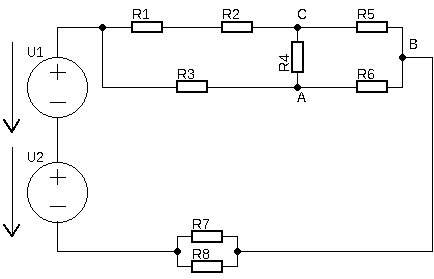
\includegraphics[width=0.6\linewidth]{img0.png}
\end{figure}
	
	{\Large Řešení (metoda postupného zjednodušování):}\\
	\begin{figure}[H]
		%\vspace{-1.1cm}
		\center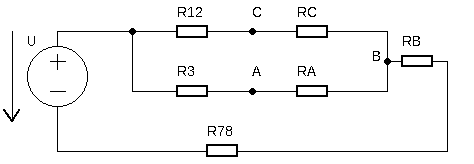
\includegraphics[width=1.1\linewidth]{img1.png}
		\caption*{Transfigurace - trojúhelník \textrightarrow \hspace{0.1cm} hvězda}
\end{figure}
\begin{gather*}
		U = U_1 + U_2 = 95 + 115 = 210 \text{V}\\[0.2cm]
		R_A = \frac{R_4  R_6}{R_4 + R_5 + R_6} = \frac{330 \cdot 830}{330 + 410 + 830} = \frac{27390}{157} \doteq 174.4586 \Omega \\
		R_B = \frac{R_5  R_6}{R_4 + R_5 + R_6} = \frac{410 \cdot 830}{330 + 410 + 830} =
\frac{34030}{157} \doteq 216.7516 \Omega \\ 
		R_C = \frac{R_4  R_5}{R_4 + R_5 + R_6} = \frac{330 \cdot 410}{330 + 410 + 830} = \frac{13530}{157} \doteq 86.1783 \Omega\\
		R_{78} = \frac{R_7 R_8}{R_7+R_8} = \frac{340 \cdot 220}{340 + 220} = \frac{935}{7}  \doteq 133.7514 \Omega
\end{gather*}
\begin{figure}[H]
		\center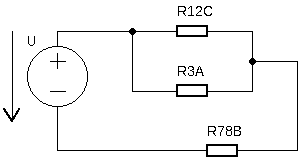
\includegraphics[width=0.6\linewidth]{img2.png}
		\caption*{$R_{12}$ a $R_C$ jsou zapojeny sériově stejně jako $R_3$ a $R_A$ a  stejně $R_{78}$ a $R_B$}
\end{figure}
\begin{gather*}
	R_{12C} = R_{12} + R_C = 1380 + \frac{13530}{157} = \frac{230190}{157} \doteq 1460.1783 \Omega \\
	R_{3A} = R_3 + R_A = 340 + \frac{27390}{157} = \frac{80770}{157} \doteq 514.4586 \Omega \\
	R_{78B} = R_{78} + R_B = \frac{935}{7} + \frac{34030}{157} = \frac{385005}{1099} \doteq 350.3230 \Omega \\
\end{gather*}
\begin{figure}[H]
		\center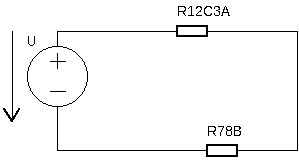
\includegraphics[width=0.6\linewidth]{img3.png}
		\caption*{$R_{12C}$ a $R_{3A}$ jsou zapojeny paralelně}
\end{figure}
\begin{gather*}
	R_{123C3A} = \frac{R_{12C} R_{3A}}{R_{12C} + R_{3A}} = \frac{\frac{230190}{157}\cdot\frac{80770}{157}}{\frac{230190}{157} + \frac{80770}{157}} = \frac{929622315}{2441036} \doteq 380.8311 \Omega
\end{gather*}
\begin{figure}[H]
\center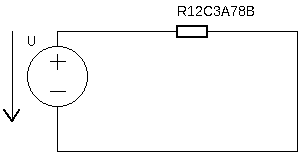
\includegraphics[width=0.6\linewidth]{img4.png}
		\caption*{$R_{12C3A}$ a $R_{78B}$ jsou zapojeny sériově}
\end{figure}
\begin{gather*}
	R = R_{12C3A} + R_{78B} = \frac{929622315}{2441036} + \frac{385005}{1099} = \frac{79575885}{108836} \doteq 731.1541 \Omega \\[0.2cm]
	I = \frac{U}{R} = \frac{210}{\frac{70247085}{2441030}} = \frac{1523704}{5305059} \doteq 0.2872172 \text{A}
\end{gather*}
\begin{figure}[H]
		\center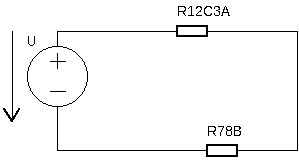
\includegraphics[width=0.6\linewidth]{img3.png}
		\caption*{$R_{12C3A}$ a $R_{78B}$ jsou zapojeny sériově}
\end{figure}
\large{Z I. Kirchhoffova zákona:}
\begin{gather*}
	I_{R_{78B}} = I_{R_{12C3A}} = I \\[0.2cm]
	U_{R_{12C3A}} = R_{12C3A} \cdot I = \frac{1523704}{5305059}\cdot\frac{929622315}{2441036} = \frac{30367662290}{277631421} \doteq 109.3812\text{V}
\end{gather*}
\begin{figure}[H]
		\center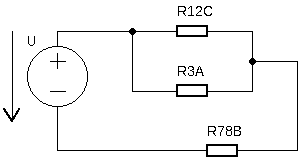
\includegraphics[width=0.6\linewidth]{img2.png}
		\caption*{$R_{12C}$ a $R_{3A}$ jsou zapojeny paralelně}
\end{figure}
\begin{gather*}
	I_{R_{3A}} = \frac{U_{R_{12C3A}}}{R_{3A}} = \frac{\frac{30367662290}{277631421}}{\frac{80770}{157}} = \frac{375977}{1768353} \doteq 0.2126142\text{A}
\end{gather*}
\begin{figure}[H]
		%\vspace{-1.1cm}
		\center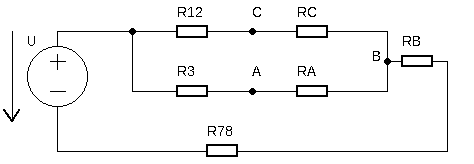
\includegraphics[width=1.1\linewidth]{img1.png}
		\caption*{$R_3$ a $R_A$ jsou zapojeny sériově}
\end{figure}
\begin{gather*}
	I_3 = I_{R_3} = \frac{375977}{1768353} \doteq 0.2126142\text{A}\\[0.2cm]
	U_{R_3} = R_3 \cdot I_{R_3} = 340 \cdot \frac{375977}{1768353} = \frac{127832180}{1768353} \doteq 72.288836\text{V}
\end{gather*}
\pagebreak
\section{Příklad (E)}
\Large{Zadání:} \\
	$U = 250 \text{V}$ \\
	$R_1 = 150 \Omega \; R_2 = 335 \Omega \; R_3 = 625 \Omega \;
	R_4 = 245 \Omega \\ R_5 = 600 \Omega $\\
	$U_{R_1} = \: \text{?}$ \\
	$I_{R_1} = \: \text{?}$ \\
\begin{figure}[H] 
		%\vspace{-1.1cm}
		\center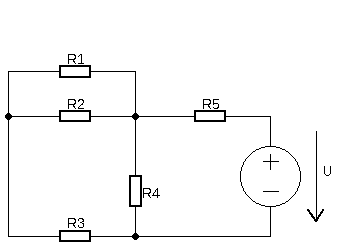
\includegraphics[width=0.6\linewidth]{img5.png}
\end{figure}
\pagebreak
	{\Large Řešení (Metoda Théveninovy věty):}\\
	\begin{figure}[H]
		 Vypočítáme $\boldsymbol{R_i}$:\\
		\center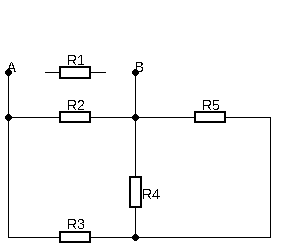
\includegraphics[width=0.6\linewidth]{img6.png}
		\caption*{Odpojíme $R_1$ a zkratujeme napěťový zdroj}
\end{figure}
\begin{gather*}
		R_i = \frac{R_2(R_3+\frac{R_4 R_5}{R_4 + R_5})}{R_2+(R_3+\frac{R_4 R_5}{R_4 +R_5})} = \frac{335\cdot(625+\frac{245\cdot600}{245+600})}{335+(625+\frac{245\cdot600}{245+600})}\doteq236.03306\Omega
\end{gather*}
\pagebreak
	\begin{figure}[H]
		\center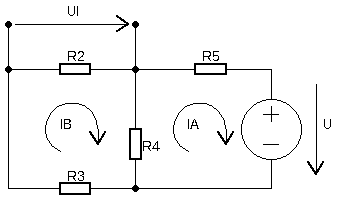
\includegraphics[width=0.6\linewidth]{img7.png}
		\caption*{Vypočítáme $I_B$ metodou smyčkových proudů}
\end{figure}
\begin{eqnarray*}
	I_AR_4+I_AR_5-I_BR_4+U &= & 0\\
	I_BR_3+I_BR_2+I_BR_4-I_AR_4 &= & 0\\\\
	245 I_A + 600 I_A-245 I_B &= & 0\\
	625I_B+335I_B+245I_B-245I_A &= & 0\\\\
	1205I_B - 245I_A &= & 0\\
	I_A&= &-\frac{50+49I_B}{169}\\\\
	1205I_B-245\bigg( -\frac{50+49I_B}{169}\bigg) &= & 0\\\\
	I_B &=& -\frac{1225}{19164}	
\end{eqnarray*}
	\begin{figure}[H]
		\center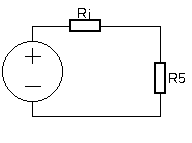
\includegraphics[width=0.6\linewidth]{img8.png}
		\caption*{Vypočítáme $U_i$ a $I_i$}
\end{figure}
\begin{gather*}
	|I_B|=\frac{1225}{19164}\doteq0.0639219\text{A}\\[0.1cm]
	U_i = R_2I_B = 335\cdot\frac{1225}{19164} = \frac{410375}{19164}\doteq21.4139\text{V}\\[0.1cm]
	I_i = \frac{U_i}{R_i+R_1}=\frac{21.4138}{236.0331+150}\doteq0.0554714\text{A}\\[0.1cm]
	I_{R_1} = I_i\doteq0.0554714\text{A}\\
	U_{R_1} = I_{R_1}R_1 = 0.0554714\cdot150\doteq8.32071\text{V}
\end{gather*}
\end{document}